\documentclass{article}

\usepackage{natbib}
\usepackage[sc]{mathpazo}
\usepackage[T1]{fontenc}
\usepackage{amsmath}
\usepackage{amsfonts}
\usepackage{amssymb}
\usepackage{graphicx}
\usepackage[onehalfspacing]{setspace}
\usepackage{color}
\usepackage[margin=.75in, tmargin=0.71in, bmargin=0.71in]{geometry}
\usepackage{url}

\usepackage{appendix}
\usepackage{hyperref}
\usepackage{xcolor}
\usepackage{todonotes}
\usepackage{booktabs}
\usepackage{lscape}
\usepackage{caption}%
\usepackage{bbm}
\usepackage{comment}

\usepackage{longtable}

\usepackage{subcaption}

\usepackage{babel}
\usepackage[autostyle, english = american]{csquotes}
\MakeOuterQuote{"}

\title{Textual Analysis and Financial Statements}
\author{Isaac Liu}

\setlength{\parindent}{0pt}
\setlength{\parskip}{0.5em}

\hypersetup{
    colorlinks=true,
    linkcolor=black,
    filecolor=black,      
    urlcolor=blue,
    citecolor=black
}

\begin{document}

	\maketitle

    \section*{Introduction}

    high-level subject area info

    \citep{das_credit_2023}

    problem statement and question

    Can incorporating the text of earnings calls improve predictions of corporate credit ratings?

    Company ratings and creditworthiness are important information for investors - not just institutional investors and financially sophisticated bondholders, but also stockholders, who may be wiped out completely in the event of bankruptcy.

    Are ratings based on hard numbers, or do company outlooks and sentiment also matter? Are they predictable?

    note credit rating data access is limited and our model can be used to interpolate

    high level data description

    roadmap
    we then

    \section*{Data and Exploratory Data Analysis}

    sources

    all data formats come as CSV though we use parquet files for efficient intermediate data storage throughout the project

    \subsection*{Credit Ratings}

    Long-term credit rating issuances from S and P Rating Services, 2010-2016

    Combination of Kaggle datasets

    Can be a change in rating (upgrade, downgrade) or reaffirmation

    Finer grades (+, -) sometimes assigned but removed for this project

    BBB and above is investment grade (one-year default ~0 to 1\%), below is junk (1 to 30, 40, 50\%)

    \begin{figure}[h!]
		\centering
        \caption{Credit Ratings}
        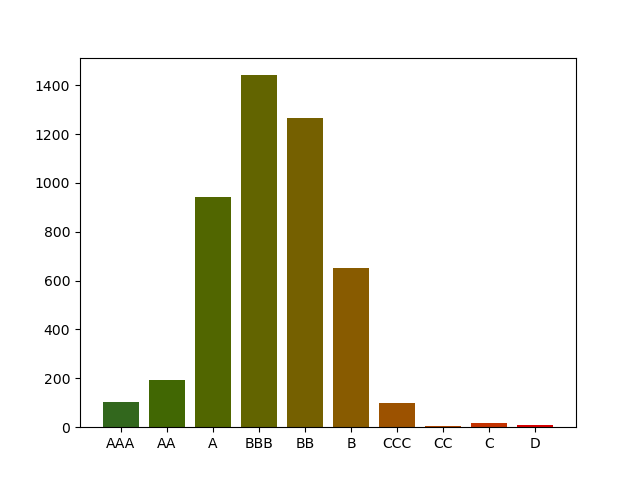
\includegraphics[width=0.5\linewidth,keepaspectratio=true]{../Output/All Data EDA/Tabular EDA/Distribution of Rating Issuances_no_title.png}
	\end{figure}

    \subsection*{Earnings Calls}

    API source

    Quarterly conference call transcripts that contains speaker remarks and Q and A session from 2010 - 2016.

    Remove all calls that happened more than 250 days prior and after the fixed quarter date

    \begin{figure}[h!]
		\centering
        \caption{Number of Words in Earnings Calls}
        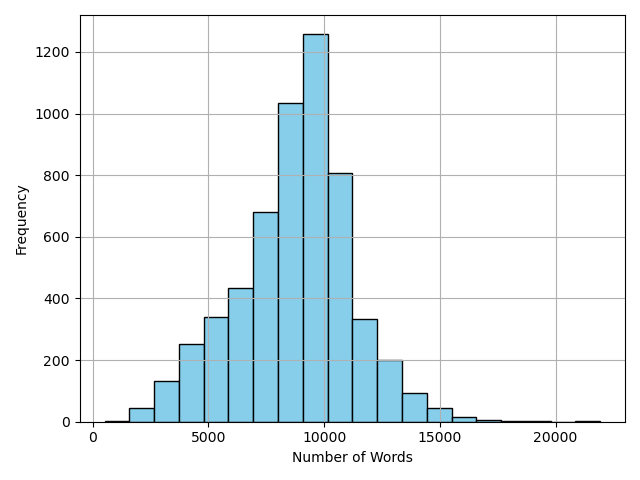
\includegraphics[width=0.5\linewidth,keepaspectratio=true]{../Output/All Data EDA/NLP EDA/all_data_num_words_distribution_no_title.png}
	\end{figure}

    \subsection*{Financial Statements}

    API source

    Items from balance sheet, cash flow statement, income statement, and company market capitalization
    
    124 variables in total. Examples: revenue, total liabilities, net income, EBITDA
    
    Limit to items reported in USD
    
    Winsorizing: Check for items mis-multiplied by 1,000 in parsing - if last digits are “000.00” and item is above or below 2.5\% and 97.5\% quantile, divide by 1,000

    Tests to ensure the value in income statement and balance sheet are consistent with each other.

    Construct Altman Z-score

    \begin{figure}[h!]
		\centering
        \caption{Altman Z-Score}
        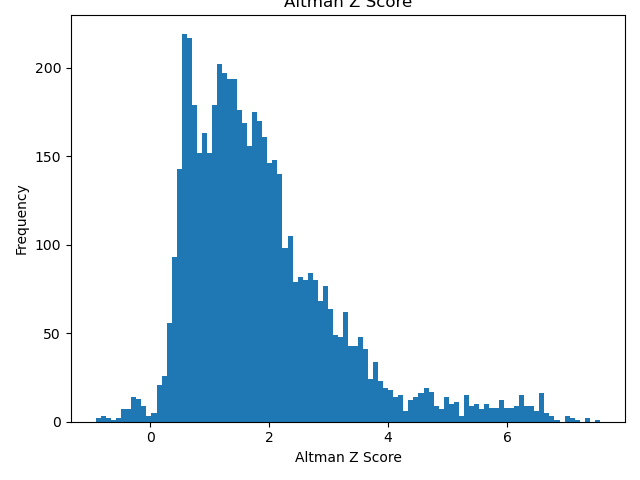
\includegraphics[width=0.5\linewidth,keepaspectratio=true]{../Output/All Data EDA/Tabular EDA/altman_z_score_all_data.png}
	\end{figure}    

    \subsection*{Sector}

    GCIS developed by S and P

    Obtained from Kaggle with supplementary manual lookup

    \begin{figure}[h!]
		\centering
        \caption{Firms by Sector}
        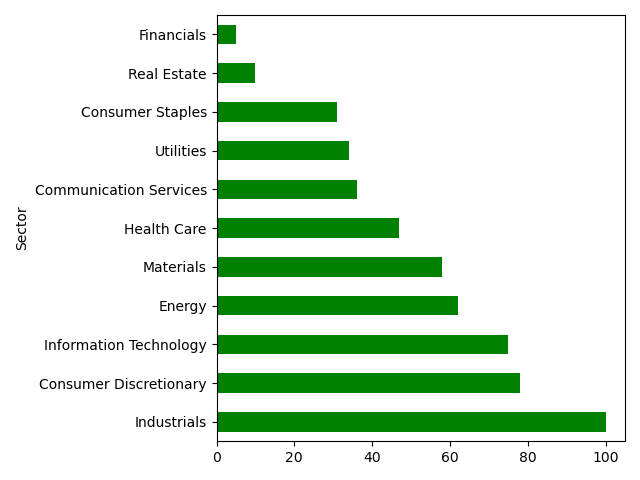
\includegraphics[width=0.5\linewidth,keepaspectratio=true]{../Output/All Data EDA/Tabular EDA/all_data_fixed_quarter_dates_firms_by_sector_no_title.png}
	\end{figure}

    sectoral imbalance

    \subsection*{Merged Data}

    Data is at the level of

    XXX quarters, XXX companies

    temporal imbalance

    \begin{figure}[h!]
		\centering
        \caption{Observations by Quarter and Year}
        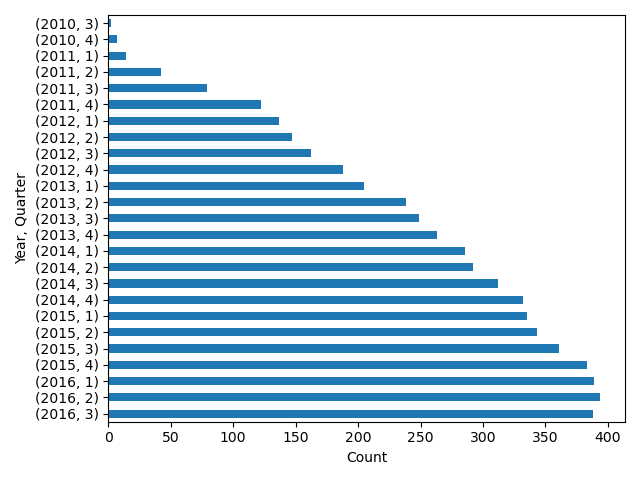
\includegraphics[width=0.5\linewidth,keepaspectratio=true]{../Output/All Data EDA/Tabular EDA/all_data_fixed_quarter_dates_obs_by_year_quarter_no_title.png}
	\end{figure}

    \subsection*{Quality Control}

    quality control
    code review of all data cleaning code
    numerous investigations

    \section*{NLP Features}

    Average call length

    \begin{figure}[h!]
		\centering
        \caption{Average Call Length by Credit Rating}
        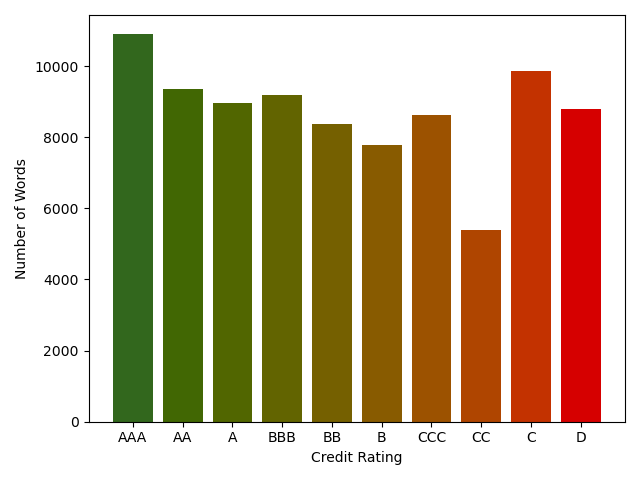
\includegraphics[width=0.5\linewidth,keepaspectratio=true]{../Output/All Data EDA/NLP EDA/all_data_call_length_by_credit_rating_no_title.png}
	\end{figure}

    outliers and errors

    correlations and patterns

    identification of good machine learning methods

    \section*{Modelling}

    Our overall model architecture is of the form

    \begin{equation*}
        \hat{\text{Credit Rating}} = f(\text{Financial Statement Variables}, \text{Sector}, \text{NLP Features})
    \end{equation*}

    functions began with logistic regression

    XXX logistic regression predictors

    multinomial, balanced class weights, l1 penalty

    table of predictions

    fitting and output

    assumptions
    
    interpretation

    \section*{Next Steps}

    Ensembling and Auto-ML

    more classifiers
    
    first steps using AutoML

    a good starting point for diving deep on more algorithms

    algorithms and accuracy from them

    outputted feature importance

    Graph Neural Network incorporating the relationships between companies, trained end-to-end with both tabular financial data and NLP features
    
    \begin{figure}[h!]
		\centering
        \caption{Company Mentions}
        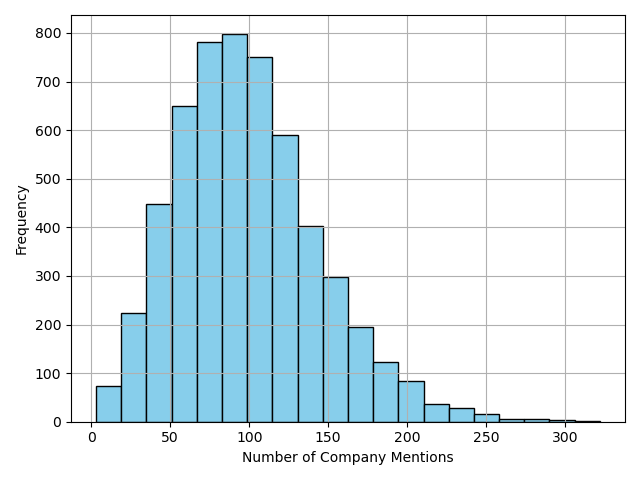
\includegraphics[width=0.5\linewidth,keepaspectratio=true]{../Output/All Data EDA/NLP EDA - NER on Company Names/Company Mentions Distribution No Title.png}
	\end{figure}

    Fine tune the pre-trained LLMs for NLP feature construction
    
    \clearpage
    \newpage

    \bibliographystyle{chicago}
    \bibliography{Stat-222-Capstone}

    \clearpage
    \newpage

    \appendix

    \section*{Appendix}

\end{document}
